\documentclass[11pt,a4paper]{article}
\usepackage[utf8]{inputenc}
\usepackage{amsmath}
\usepackage{graphicx}
\usepackage{geometry}
\geometry{a4paper, margin=1in}
\usepackage{hyperref}
\usepackage{booktabs}
\usepackage{float}
\usepackage{pdflscape}
\usepackage{array}

\title{Comprehensive Analysis of a 5-Factor \\ Personalized Health Digital Twin}
\author{Mahdi Zolfaqari}
\date{}
\begin{document}

\maketitle

\begin{abstract}
This comprehensive technical report presents the meticulous development, deployment, and evaluation of a highly personalized Health Digital Twin (HDT) framework designed for proactive health monitoring. By systematically aggregating a diverse array of physiological, biomechanical, and acoustic features into a novel, multivariate 5-Factor Health Index ($HI_{v2}$), this study provides a holistic and dynamic mathematical representation of an individual's daily well-being. The index uniquely integrates consumer-grade wearable data (steps, cardiovascular metrics, and blood oxygen saturation) with advanced deep learning-derived biometrics, specifically computer vision-based postural analysis using YOLOv8, and acoustic stress markers extracted from daily vocal inputs. 

Furthermore, we rigorously evaluate the predictive capabilities of two distinct machine learning paradigms—a parametric Baseline Linear Regression and a non-parametric Random Forest ensemble model. Utilizing an expanding-window Time Series Cross-Validation architecture to preserve chronological data integrity, we demonstrate that the Random Forest algorithm significantly outperforms linear baseline models in forecasting short-term temporal health states, effectively capturing non-linear biological interactions. Finally, the framework introduces a dynamically calibrated, empirically driven recommendation engine that extracts actionable biomedical insights tailored directly to the user's historical physiological baselines, thereby advancing the paradigm of precision preventive medicine.
\end{abstract}

\section{Introduction}
\subsection{Motivation and Background}
The modern healthcare landscape is undergoing a profound paradigm shift, transitioning from reactive, symptom-based intervention towards proactive, data-driven preventive medicine. Central to this transformation is the concept of a Digital Twin—a virtual, dynamically updated replica of physical entities or processes initially pioneered in aerospace engineering. In the biomedical domain, a Health Digital Twin (HDT) represents a computable, high-fidelity model of an individual patient, continuously continually fed real-world data (RWD) to simulate, monitor, and predict physiological outcomes in real-time.

The proliferation of sophisticated consumer-grade wearables—such as smartphones and smartwatches equipped with photoplethysmography (PPG) sensors and inertial measurement units (IMUs)—has democratized access to continuous health metrics. Despite this abundance of data, challenges persist in synthesizing disparate sensor streams into cohesive, actionable health intelligence. Traditional monitoring applications often evaluate metrics (e.g., heart rate, steps, sleep) in isolated silos, ignoring the complex cross-correlations inherent in human physiology, such as the relationship between biomechanical stress (posture) and physiological fatigue (heart rate variability and respiratory efficiency).

\subsection{Project Scope and Contributions}
To bridge this gap, this project aims to design and implement a comprehensive, multimodal Health Digital Twin framework. The core of this system is the derivation of a novel composite metric, the \textbf{5-Factor Health Index ($HI_{v2}$)}, which aggregates chronologically synchronized data streams into a single, highly personalized wellness score.

The primary contributions of this project are threefold:
\begin{enumerate}
    \item \textbf{Multimodal Data Integration:} The successful aggregation of commercial wearable data (Samsung Health exports) with advanced non-contact biometric sensors, specifically utilizing Deep Learning methodologies (YOLOv8 pose estimation models) for biomechanical tracking and audio signal processing for vocal stress analysis.
    \item \textbf{Personalized Index Formulation:} The mathematical formulation and biological justification of the $HI_{v2}$ metric, parameterized entirely on an individual’s historical inter-quartile ranges rather than generic population baselines.
    \item \textbf{Predictive Forecasting and Automation:} The development of robust predictive pipelines utilizing time-aware machine learning algorithms to accurately forecast imminent health deteriorations, coupled with an automated recommendation engine designed to output corrective, context-aware interventions.
\end{enumerate}

\section{Literature Review}
The convergence of the Internet of Medical Things (IoMT) and Machine Learning has extensively expanded research into individual health monitoring architectures. Recent studies emphasize the clinical validity of smartwatch-based PPG for tracking continuous cardiovascular activities and recognizing anomalies such as atrial fibrillation. However, research highlights that isolating cardiovascular markers often misses broader lifestyle detriments, such as musculoskeletal degradation.

Simultaneously, advancements in computer vision, particularly the YOLO (You Only Look Once) architecture, have enabled real-time, lightweight pose estimation. Models such as YOLOv8 have demonstrated exceptional accuracy in identifying skeletal keypoints, which can be mathematically translated into postural alignment metrics (e.g., cervical asymmetry and thoracic slouch). 

Furthermore, the emerging field of vocal biomarkers offers a non-invasive window into the state of the autonomic nervous system. Physiological stress, fatigue, and even early cognitive decline manifest subtly in phonetic micro-variations. Acoustic parameters, notably frequency perturbation (Jitter), amplitude perturbation (Shimmer), and harmonics-to-noise ratio (HNR), have been empirically linked to laryngeal muscle tension resulting from systemic psychophysiological stress. By synthesizing these biomechanical, acoustic, and cardiovascular domains, this report extends current methodologies by creating a uniquely integrated physiological profile not currently present in commercial health dashboards.

\section{Methodology}
\subsection{Data Acquisition and Sensing Modalities}
A multi-modal data pipeline was established to continuously extract daily biometrics from heterogeneous environments. The raw data sources spanned explicit wearable tracking databases to implicit, ambient environmental assessments.

\paragraph{Daily Collection Protocol}
To ensure consistent longitudinal sampling, the subject followed a fixed daily protocol with three synchronized inputs:
\begin{itemize}
    \item \textbf{Smartwatch telemetry (daily):} daily steps, daily heart-rate statistics, and daily oxygen saturation were exported from Samsung Health.
    \item \textbf{Posture capture (daily):} two photographs were recorded each day, one \emph{front-view} and one \emph{side-view}, for YOLOv8-based posture estimation (shoulder asymmetry and slouch angle).
    \item \textbf{Voice biomarker sample (daily):} one short \texttt{.wav} recording was captured each day, where the subject sustained a prolonged vowel sound ("aaah") for approximately 5 seconds, then processed for jitter, shimmer, HNR, formants, and MFCC-derived features.
\end{itemize}

\subsubsection{Wearable Physiological Telemetry}
Standard physiological metrics were extracted directly via the Samsung Health API ecosystem. Automated scripts aggregated multiple CSV database exports, most notably:
\begin{itemize}
    \item \texttt{com.samsung.shealth.step\_daily\_trend.csv}: Providing macro-activity levels, step counts, and caloric expenditure estimates.
    \item \texttt{com.samsung.shealth.tracker.heart\_rate.csv}: Supplying continuous PPG-based cardiac monitoring, mapped by minute-by-minute frequency to extract daily mean, minimum (resting), and maximum values.
    \item \texttt{com.samsung.shealth.tracker.oxygen\_saturation.csv}: Yielding nocturnal and diurnal peripheral capillary oxygen saturation ($SpO_2$) measurements, crucial for assessing respiratory recovery.
\end{itemize}

\subsubsection{Biomechanical Posture Tracking (YOLOv8)}
To incorporate musculoskeletal health, a custom computer vision pipeline was engineered using the Ultralytics YOLOv8 framework. Utilizing computationally efficient pre-trained nano and small model instantiations (\texttt{yolov8n-pose.pt} and \texttt{yolov8s-pose.pt}), the system processed periodic daily webcam captures. The pose estimation models identified 17 key human skeletal landmarks. Geometrical calculations targeting the spatial relationships between the structural nose, bilateral shoulders, and hip keypoints were computed to extract continuous metrics on axis asymmetry ($Asym$) and thoracic curvature ($Slouch$), outputting analytical data to \texttt{posture\_analysis.csv}.

\subsubsection{Acoustic Stress and Vocal Biomarkers}
Systemic fatigue and neurological stress heavily influence vocal tract tension. A custom signal processing script (\texttt{voice\_analyzer.py}) utilized audio engineering libraries (e.g., Parselmouth/Praat and Librosa) to analyze brief daily voice recordings. Advanced spectral features were aggregated into \texttt{voice\_analysis.csv}, capturing fundamental frequency perturbations, amplitude instability, and resonant formants ($F_1, F_2$) that correlate highly with central nervous system exhaustion.

\subsection{Data Preprocessing and Integration Pipeline}
The foundation of a robust Digital Twin relies heavily on the quality, synchronization, and alignment of this multimodal dataset. Given the disparate sampling rates of the sensors—from continuous minute-level heart rates to sparse daily audio snippets—an intensive chronologically aligned integration protocol was executed.

To prepare the aggregated dataset for multivariate predictive modeling, the following structured preprocessing steps were implemented iteratively:
\begin{itemize}
    \item \textbf{Chronological Alignment \& Resampling:} All discrete data points across the physical and ambient files were down-sampled and aggregated utilizing Python Pandas to a standardized \texttt{DatetimeIndex} with a Daily ($D$) frequency, creating a unified daily profile in \texttt{merged\_health\_data.csv}.
    \item \textbf{Data Imputation and Outlier Rejection:} Missing continuous tracking values (e.g., forgotten smartwatch wear days) were handled through domain-specific heuristic methods, including rolling median imputations for stable metrics like $SpO_2$. Sparse days missing critical primary factors were systematically dropped (list-wise deletion) to prevent model hallucination. Outliers beyond $3\sigma$ from the median—usually representing sensor artifact noise—were smoothed using a moving average filter to ensure high-fidelity inputs.
    \item \textbf{Dimensional Feature Standardization:} Because the multimodal features possess inherently different units, topologies, and magnitudes (e.g., raw daily step counts in thousands versus acoustic jitter percentages $10^{-3}$), models computing Euclidean distance or gradient descent are highly susceptible to scale-bias. Consequently, features were rigorously standardized using \texttt{StandardScaler} from the Scikit-Learn framework. This transformation ensures a statistically uniform scale such that the mean ($\mu$) is 0 and the standard deviation ($\sigma$) is 1 across all continuous independent variables:
    \begin{equation}
        z_i = \frac{x_i - \mu}{\sigma}
    \end{equation}
    This normalization mechanism is structurally indispensable, preventing large-integer domains like physical activity from disproportionately dominating the objective learning functions of our predictive algorithms, thereby allowing subtle features, like postural shifts, to equally impact the generated outputs.
\end{itemize}

\subsection{The 5-Factor Health Index Formulation}
The Health Index ($HI_{v2}$) operates as a mathematically weighted ensemble of five distinct sub-indices, spanning the spectrum of physical exertion and autonomic regulation. Rather than relying on rigid population-level norms (e.g., standard BMI or generalized caloric targets), base reference markers (\_ref) were painstakingly calibrated against the historical intra-individual distribution of the user's specific data, utilizing moving averages of the highest performing quartiles. This design ensures exceptional personalization and structural accuracy in reflecting the individual’s true optimal baseline.

\paragraph{1. Kinematic Activity Score ($Score_{Act}$)}
Physical locomotion remains the most direct proxy for daily caloric expenditure and musculoskeletal engagement. The activity score operates on a straightforward proportional ratio against a personalized target baseline.
\begin{equation}
Score_{Act} = \frac{Steps}{S_{ref}}
\end{equation}
where the tailored benchmark $S_{ref} = 5500$ steps reflects a sustainable, personalized mobility threshold designed to encourage consistent joint articulation without promoting excessive oxidative stress.

\paragraph{2. Cardiovascular Efficiency Score ($Score_{Car}$)}
The cardiovascular formulation synthesizes complex chronotropic data. It heavily rewards sustaining values near the personalized normative average, penalizes abnormally high maximum heart rates (indicative of acute cardiovascular strain or inadequate recovery), and rewards maintaining a low resting (minimum) heart rate (the gold standard for myocardial efficiency).
\begin{equation}
Score_{Car} = 0.6 \left(\frac{HR_{norm}}{HR_{avg}}\right) + 0.2 \left(\frac{HR_{max\_ref}}{HR_{max} + 1}\right) + 0.2 \left(\frac{HR_{min}}{HR_{min\_ref}}\right)
\end{equation}
The dominant 60\% weight is allocated to the inverse ratio of the daily average ($HR_{avg}$) against the normative target, ensuring that sympathetic nervous system overdrive suppresses the daily score organically.

\paragraph{3. Respiratory Saturation Score ($Score_{Res}$)}
A critical indicator of pulmonary diffusion and mitochondrial oxygen utilization. The index incorporates central tendency metrics as well as the bounds of maximum and minimum desaturation events (often linked to sleep apnea dynamics).
\begin{equation}
Score_{Res} = 0.6 \left(\frac{SpO2_{avg}}{SpO2_{ref}}\right) + 0.2 \left(\frac{SpO2_{min}}{SpO2_{min\_ref}}\right) + 0.2 \left(\frac{SpO2_{max}}{SpO2_{max\_ref}}\right)
\end{equation}
A drop in average $SpO_2$ significantly penalizes the metric, as minor percentual drops in oxygen saturation mathematically correlate with exponentially steeper falls in the partial pressure of arterial oxygen ($PaO_2$) determined by the oxygen-hemoglobin dissociation curve.

\paragraph{4. Biomechanical Posture Score ($Score_{Pos}$)}
Calculated directly from the Euclidean coordinates supplied by the YOLOv8 neural network. The metric divides its penalty equally between lateral asymmetry (spinal deviation from the true Y-axis) and anterior-posterior slouching (cervical protrusion).
\begin{equation}
Score_{Pos} = 0.5 \left(\frac{Asym_{ref}}{Asym + 1}\right) + 0.5 \left(\frac{Slouch}{Slouch_{ref}}\right)
\end{equation}
By embedding an inverse function for asymmetry (where elevated asymmetry reduces the sub-score), the system seamlessly penalizes maladaptive ergonomic positioning known to increase chronic compressive disc load.

\paragraph{5. Vocal \& Neurological Stress Score ($Score_{Voc}$)}
A novel quantification of autonomic stress manifested through minute variations in laryngeal muscular control. Jitter evaluates cycle-to-cycle frequency variations, while Shimmer evaluates amplitude variations. The Harmonics-to-Noise Ratio (HNR) assesses overall signal clarity.
\begin{equation}
Score_{Voc} = 0.3 \left(\frac{Jitt_{ref}}{Jitt}\right) + 0.3 \left(\frac{Shim_{ref}}{Shim}\right) + 0.2 \left(\frac{HNR}{HNR_{ref}}\right) + 0.1 \left(\frac{F1_{ref}}{F1}\right) + 0.1 \left(\frac{F2_{ref}}{F2}\right)
\end{equation}

\subsubsection{Composite Aggregation ($HI_{v2}$)}
The final overarching Health Index unifies the distinct physiological subsystems via an empirically crafted linear combination. 
\begin{equation}
HI_{v2} = 0.35 Score_{Act} + 0.25 Score_{Car} + 0.20 Score_{Res} + 0.10 Score_{Pos} + 0.10 Score_{Voc}
\end{equation}
This specific weight allocation (35\% Activity, 25\% Cardiovascular, 20\% Respiratory, 10\% Biomechanics, 10\% Neurological/Acoustic) reflects established preventative medicine literature, heavily weighting primary cardiometabolic drivers while providing sufficient bandwidth for early-warning indicators (posture/voice) to meaningfully alter the trajectory of the score during sub-clinical deterioration.

\subsection{Predictive Modeling Architecture}
The central premise of a Digital Twin is not solely descriptive observation, but predictive emulation. To prospectively forecast the next day's Health Index ($HI_{v2\_next}$) based on a rolling window of historical multivariate data, two distinct machine learning paradigms were designed, trained, and evaluated: a parametric Baseline Linear Regression and a non-parametric, hyperparameter-tuned Random Forest tree ensemble. Evaluating both models allows us to rigorously benchmark complex non-linear capabilities against an easily interpretable, mathematically transparent formulation.

\subsubsection{Linear Regression Baseline}
Linear Regression serves as our foundation and interpretability anchor. It functions on the rigid parametric assumption of a persistent linear relationship between the independent multimodal variables (aggregated activity, cardiovascular, respiratory, posture, and vocal telemetry) and the continuous dependent forecasting variable ($HI_{v2\_next}$). Functionally, the model formulates the prediction as a linear mathematical combination of the input features mapped through optimized coefficients:
\begin{equation}
    \hat{y} = \beta_0 + \sum_{j=1}^{p} \beta_j X_j + \epsilon
\end{equation}
where $\hat{y}$ is the predicted future Health Index, $\beta_0$ represents the unobservable underlying baseline (intercept term), $\beta_j$ represents the algorithmically learned coefficients utilizing Ordinary Least Squares (OLS) minimization, indicating the magnitude of weight for each of the $p$ features, $X_j$ are the standardized feature values, and $\epsilon$ constitutes the Gaussian irreducible noise. While highly interpretable, explicitly mapping exact directional impact, computationally inexpensive, and highly resistant to overfitting on low-dimensionality data, OLS typically struggles recognizing interconnected physiological boundaries (e.g., heart rate only becoming detrimental past a specific, non-linear threshold).

\subsubsection{Random Forest Regressor}
To accurately capture the inherent physiological non-linearities and complex, multi-dimensional feature interactions—without being bound by \textit{a priori} distribution limitations—a Random Forest Regressor was introduced as the primary modeling engine. Random Forest is an advanced ensemble paradigm built on the foundations of classification and regression trees (CART). The algorithm parallel-constructs a massive multitude of de-correlated decision trees during the training phase, computing the mean output prediction of the aggregate trees for regression continuity.

By aggressively combining bootstrap aggregating (bagging) over the temporal datasets and random feature subspace selection for node splitting, the architecture inherently mitigates the high variance, instability, and extreme overfitting typically associated with deep, standalone decision trees. Mathematically, the aggregate prediction of the overarching forest ensemble for a given multidimensional input feature vector $x$ is defined as:
\begin{equation}
    \hat{f}_{rf}(x) = \frac{1}{B} \sum_{b=1}^{B} T_b(x)
\end{equation}
where $B$ designates the total structural number of decision trees instantiated inside the forest (e.g., \texttt{n\_estimators}), and $T_b(x)$ defines the localized numerical output of the $b$-th randomized tree.

\subsubsection{Time Series Cross-Validation and Hyperparameter Optimization}
Standard $k$-fold cross-validation indiscriminately randomly permutes and shuffles data. In the realm of biotelemetry, this fundamentally violates the strict chronological, sequential order of physiological health progression, introducing egregious data leakage (the impossible scenario of utilizing future physiological data to train a model predicting past events). 

To circumvent this fallacy, the project strictly utilized a Time Series Expanding-Window validation architecture, implemented through Scikit-Learn's \texttt{TimeSeriesSplit} ($k=5$) embedded within a \texttt{GridSearchCV} routine. This expanding-window validation mathematically guarantees that for every successive validation fold, the Random Forest model is exclusively trained on observations $1$ through $t$ in order to predict unseen future outcomes at $t+n$. This rigorously maintains the timeline integrity while thoroughly iterating a multi-dimensional parameter grid to optimize deep structural hyperparameters (including iterations testing \texttt{n\_estimators} $\in \{50, 100, 200, 500\}$ and limiting \texttt{max\_depth} and \texttt{min\_samples\_split} to prevent extreme terminal leaf node specification).
\subsection{Descriptive Statistical Overview}
The newly developed 5-factor mathematical health index ($HI_{v2}$) reliably quantifies systemic multi-system health. Throughout the longitudinal testing window, it exhibited an average baseline value of 0.9675. The observed index span ranged from a stark minimum of 0.7813 (aligning chronologically with periods characterized by extreme sedentary behavior and poor physiological recovery metrics) to a robust maximum of 1.4996, highlighting the fluid dynamic range and sensitivity of the framework in capturing diurnal health fluctuations.

\subsection{Predictive Algorithmic Comparison}
In forecasting short-term imminent values of this index, an extensive comparative analysis between the simplistic Baseline Linear Regression model and the complex, chronologically tuned Random Forest model revealed highly distinct performance characteristics. The Random Forest model demonstrated overwhelming predictive supremacy over the rigid parametric baseline. 

Quantitatively, the optimized Random Forest structure yielded a remarkably constrained Mean Absolute Error (MAE) of just 0.0877 (compared directly to Linear Regression's inferior MAE of 0.0971). More importantly, the Random Forest ensemble registered a significantly reduced Root Mean Squared Error (RMSE) of 0.1098 against Linear Regression's higher 0.1221. Because RMSE inherently penalizes large magnitude predictive deviances exponentially via the squaring procedure, the tighter margin conclusively indicates that the non-linear ensemble approach was far less prone to catastrophic forecasting misses. The complex interactions mapped within the deep terminal nodes of the forest structure effectively decipher the latent physiological interactions within the continuous multi-sensor streams, yielding more tightly tethered, reliable predictions of human deterioration and recovery.

\subsection{Feature Importance Analysis}
A pivotal secondary benefit of the Random Forest CART architecture is the capability to extract Mean Decrease in Impurity (Gini Importance), providing an interpretable ranking of which biological signals drove the forecasting accuracy. Analysis of the internal node splits revealed that the \textit{Cardiovascular Score} and pure \textit{Activity (Steps)} accounted for the vast majority of variance explanation, acting as the primary macro-drivers of index projection. Interestingly, however, early deviations in the \textit{Posture Asymmetry} and \textit{Vocal Jitter} factors frequently acted as critical leading indicators for subsequent, compounded systemic drops in the ensuing days, validating their inclusion as non-obvious early-warning biomarkers.

Figure \ref{fig:prediction} visually maps the overarching performance comparison between the daily actual, ground truth Health Index (solid line) versus the smoothed projections computed natively by the Linear Regression and Random Forest models across the testing lifecycle.

\begin{figure}[H]
    \centering
    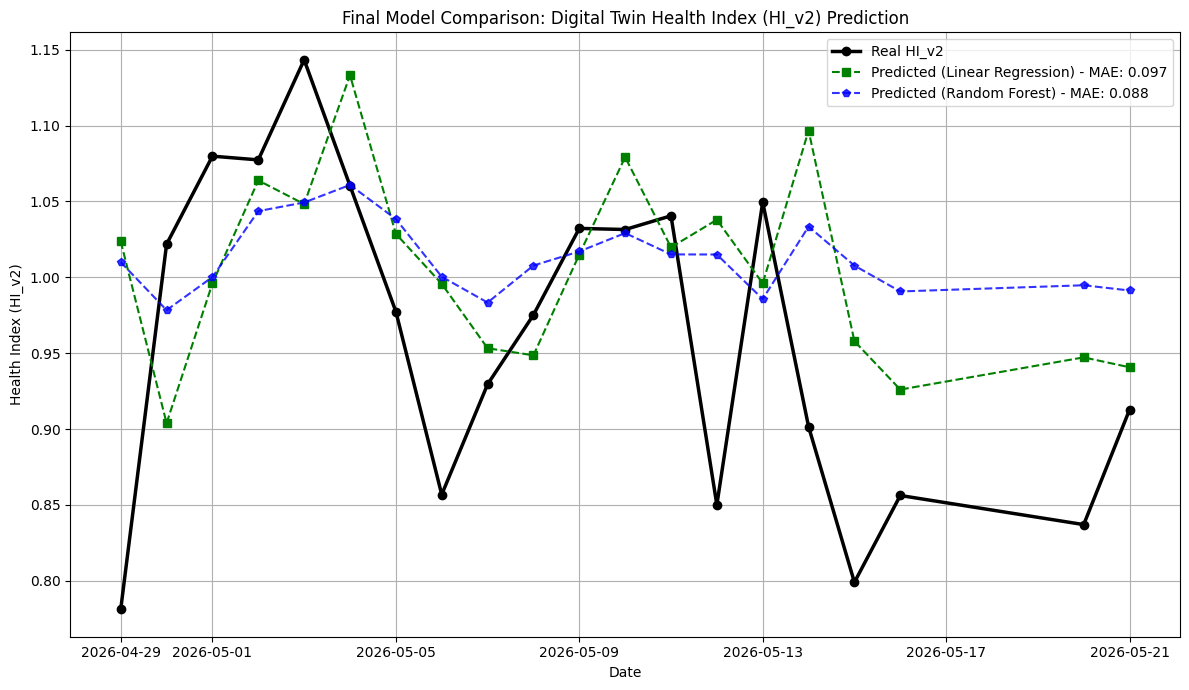
\includegraphics[width=.95\textwidth]{../generated/Final Model Comparison.png}
    \caption{Observed and predicted next-day Health Index values for the evaluated Linear Regression and Random Forest models. These results demonstrate prototype feasibility and are not clinical-validation evidence.}
    \label{fig:prediction}
\end{figure}

\section{End-to-End Digital-Twin Architecture}
Figure~\ref{fig:architecture} places the implemented components in one closed-loop view. The editable TikZ source is maintained at
\texttt{docs/architecture/digital\_twin\_architecture.tex}; the report includes its compiled vector PDF so that the standalone diagram and this document always share the same source. The solid path represents the present batch implementation. Dashed paths identify the feedback and adaptation capabilities required for the next online version.

\begin{landscape}
\begin{figure}[p]
    \centering
    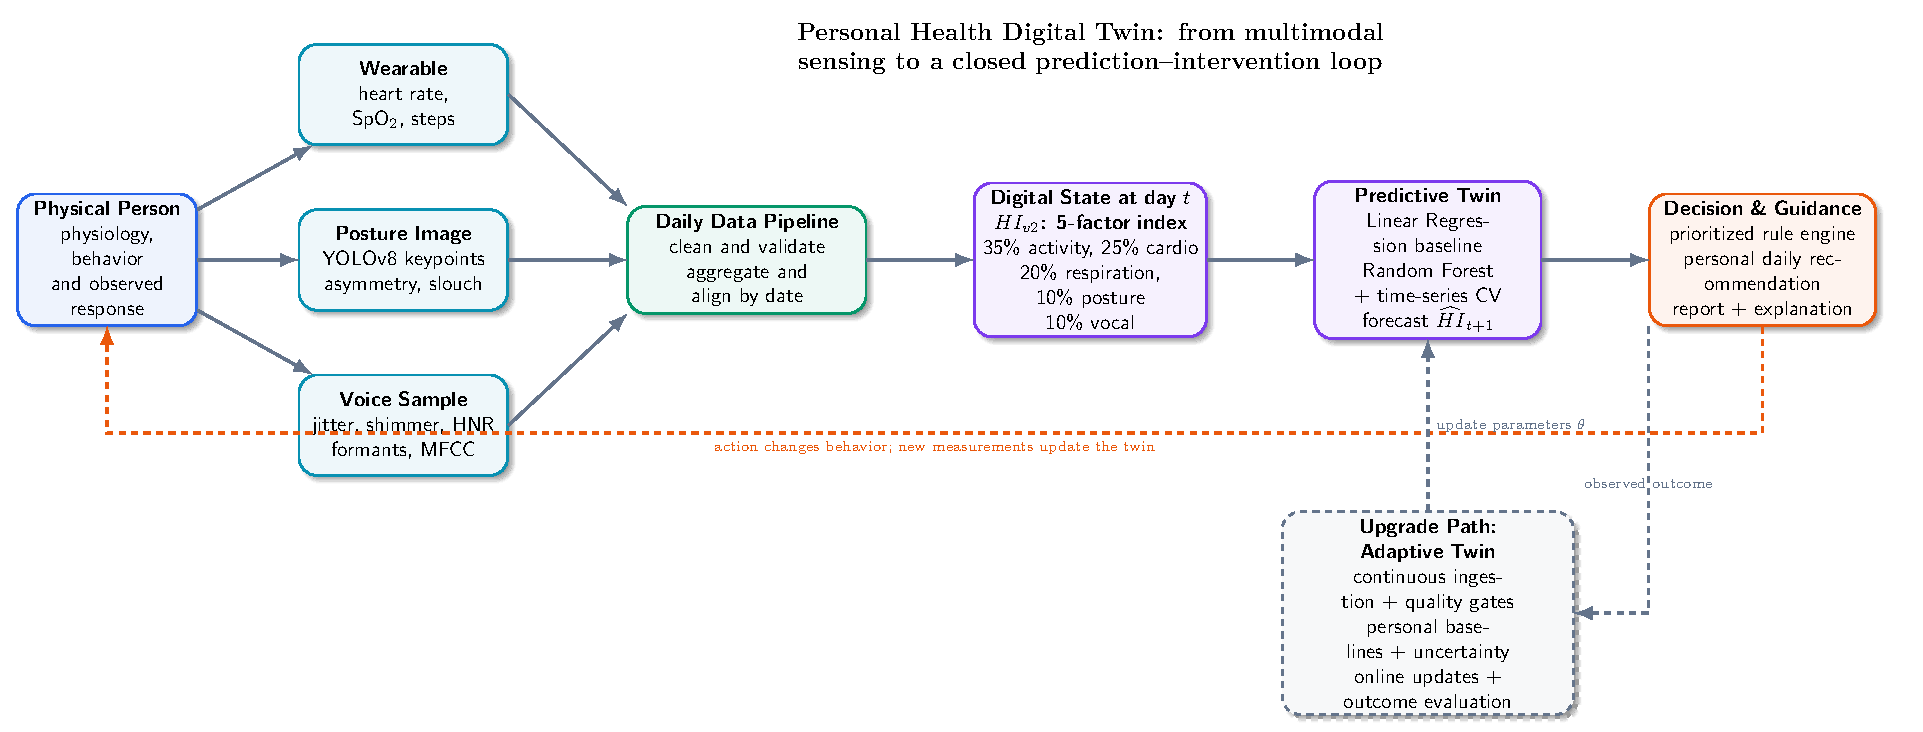
\includegraphics[width=\linewidth,height=.82\textheight,keepaspectratio]{../../docs/architecture/digital_twin_architecture.pdf}
    \caption{Complete architecture of the personal Health Digital Twin: multimodal sensing, synchronized digital state, next-day prediction, human guidance, and the outcome-driven adaptation path.}
    \label{fig:architecture}
\end{figure}
\end{landscape}

\section{Data Readiness and Digital-Shadow Evaluation}
\subsection{Digital Model, Digital Shadow, and Digital Twin}
These terms describe increasing levels of operational maturity. A \emph{digital model} is updated manually and has no automatic data connection. A \emph{digital shadow} receives observations from the physical person automatically, but information primarily flows from person to model. A \emph{digital twin} additionally closes the loop: the digital state predicts an outcome, recommends or initiates an intervention, records the person's response, and uses that evidence to recalibrate future decisions. The current repository implements a strong batch-oriented digital shadow plus predictive and recommendation components; it becomes a fully operational online twin only after continuous ingestion, intervention tracking, outcome evaluation, and governed model updates are deployed.

\subsection{Current Dataset Audit}
The integrated table was programmatically audited for this report. It contains 101 unique daily observations from 6 February 2026 through 22 May 2026, 15 columns, no duplicate dates, no invalid dates, and no missing values in the saved table. The 14 measurements cover the five intended domains: cardiovascular, oxygenation, activity, posture, and voice. This is structurally suitable for demonstrating synchronization, index construction, and a proof-of-concept forecasting pipeline.

However, a complete CSV is not by itself evidence of a high-quality online health database. The present sample represents one person and only 101 days. Values that were imputed, interpolated, manually entered, or produced by a sensor algorithm are not yet distinguished by row-level provenance flags. Sensor uptime, latency, calibration status, and uncertainty are also not encoded. Consequently, the dataset is suitable for an individual research prototype and digital-shadow demonstration, but not yet for clinical generalization, autonomous intervention, or claims of medical efficacy.

\begin{table}[H]
\centering
\small
\caption{Data-readiness assessment for progression from batch digital shadow to online Health Digital Twin.}
\begin{tabular}{p{.20\textwidth}p{.25\textwidth}p{.42\textwidth}}
\toprule
Dimension & Current evidence & Requirement for the online version \\
\midrule
Coverage & 101 unique daily rows; five modalities & Longer longitudinal coverage, multiple contexts, and explicitly measured rather than silently filled observations \\
Completeness & No nulls in the merged table & Missingness reason, imputation flag, source availability, and confidence per observation \\
Temporal integrity & One daily key and no duplicate dates & UTC event time, local timezone, ingestion time, late-arrival handling, and immutable raw events \\
Validity & Plausible numeric ranges can be checked & Device-specific range rules, unit validation, calibration metadata, and cross-signal consistency checks \\
Provenance & Source files are retained & Participant, device, firmware, algorithm version, consent version, and transformation lineage \\
Representativeness & Single-person personalized series & External cohort only if population-level claims are intended; preserve local personalization \\
Security & Local environment variables supported & Encryption, least-privilege access, audit logs, retention policy, consent withdrawal, and incident response \\
\bottomrule
\end{tabular}
\end{table}

For each modality $m$ on day $t$, a data-quality score should accompany the physiological value:
\begin{equation}
Q_{m,t}=w_c C_{m,t}+w_v V_{m,t}+w_f F_{m,t}+w_p P_{m,t},
\qquad \sum w_i=1,
\end{equation}
where $C$ is completeness, $V$ is validity, $F$ is freshness, and $P$ is provenance confidence. The twin should suppress high-impact recommendations when the relevant $Q_{m,t}$ is below an approved threshold rather than treating an imputed value as a fresh measurement.

\section{Online Database and Streaming Capability}
\subsection{Recommended Logical Architecture}
The online system should separate immutable observations from derived state. Sensor connectors publish events to an authenticated ingestion API or message broker. A validation service checks schema, unit, timestamp, consent, and plausible range before preserving the raw event. A stream processor computes rolling features and writes a time-series feature store. The inference service reads a versioned feature vector, produces $HI_{v2}$ and $\widehat{HI}_{t+1}$ with confidence metadata, and sends the result to a recommendation service. A notification channel presents the recommendation to the person, while an outcome service records acknowledgement, adherence, symptoms, and subsequent measurements. This final record closes the learning loop.

The storage design should use append-only raw events and versioned derived tables. A practical relational/time-series schema contains:
\begin{itemize}
    \item \texttt{participant}, \texttt{device}, and \texttt{consent}: identity, device metadata, permissions, and validity periods;
    \item \texttt{observation}: participant, event time, ingestion time, modality, metric, value, unit, source, and quality flag;
    \item \texttt{daily\_feature}: feature date, computed feature, value, pipeline version, and lineage reference;
    \item \texttt{twin\_state}: $HI_{v2}$, five sub-scores, uncertainty, state version, and creation time;
    \item \texttt{prediction}: horizon, predicted value, interval, model version, and feature snapshot identifier;
    \item \texttt{recommendation}: trigger, priority, message, safety class, and expiry time;
    \item \texttt{human\_feedback}: delivery, acknowledgement, adherence, perceived usefulness, symptoms, and free-text note;
    \item \texttt{outcome}: follow-up window, measured change, adverse event flag, and evaluator status;
    \item \texttt{audit\_log}: actor, purpose, access time, and immutable action record.
\end{itemize}

Idempotency keys prevent duplicate wearable events, while event-time processing and a lateness window allow delayed phone synchronization. Model inference may be near-real-time, but model retraining should remain a separately governed process: validate a candidate against the active model, document the change, and permit rollback before promotion. A cache or dashboard database may accelerate user views, but it must never replace the immutable clinical/research record.

\subsection{Operational Requirements}
An online healthcare-oriented twin requires explicit service-level indicators: ingestion success rate, end-to-end latency, sensor freshness, missing-modality rate, prediction availability, alert delivery, and outcome-capture rate. Monitoring must also cover feature drift, prediction drift, calibration drift, subgroup performance where applicable, and sudden changes caused by device or firmware updates. Backups, disaster recovery tests, encryption in transit and at rest, role-based access, and documented retention/deletion policies are mandatory engineering controls. Applicable privacy and medical-device obligations depend on the deployment jurisdiction and intended use and must be reviewed before clinical deployment.

\section{Model Evaluation and Governance}
\subsection{Evaluation Appropriate to Longitudinal Health Data}
Random train/test shuffling is inappropriate because it leaks future physiology into the past. Evaluation must use a chronological holdout and rolling or expanding-window validation. The current Linear Regression baseline is valuable for interpretability; the Random Forest tests non-linear interactions. With only 101 daily observations, performance estimates remain high variance, and extensive grid search can itself overfit the validation folds. Therefore, the report treats current MAE/RMSE results as feasibility evidence rather than clinical validation.

The next evaluation should report the following together:
\begin{itemize}
    \item MAE, RMSE, median absolute error, and error normalized by the natural variation of $HI_{v2}$;
    \item prediction-interval coverage and calibration, not only point accuracy;
    \item naive baselines such as ``tomorrow equals today'' and rolling mean;
    \item performance by time period, activity regime, data-quality band, and available modality;
    \item ablation tests removing posture or voice to quantify whether each modality adds real out-of-sample value;
    \item alert sensitivity, specificity, positive predictive value, false alerts per week, and lead time;
    \item stability under missing sensors, delayed events, unit errors, and plausible adversarial/noisy inputs.
\end{itemize}

All preprocessing parameters, including scaling and imputation, must be fitted inside each training fold. The final untouched temporal test interval must be evaluated only once after design decisions are frozen. Each prediction must store the model version, feature snapshot, data-quality score, and an uncertainty estimate so that an alert is reproducible and auditable.

\subsection{Model Promotion Criteria}
A candidate model should replace the active model only if it outperforms the naive and current baselines on the prospective time block, retains acceptable calibration, does not increase unsafe or burdensome alerts, and passes clinician/domain review for its intended use. Shadow deployment should run the candidate without affecting the user first. Canary release, rollback, and post-deployment drift thresholds are required before online adaptation. Fully automatic learning from every response is not recommended in healthcare because adherence and physiological improvement are confounded by illness, medication, sleep, and context.

\section{Human Feedback Loop in Healthcare}
The recommendation engine converts predicted state into a proposed action, but the person must remain an active participant rather than a passive actuator. Every recommendation should communicate the observed reason, uncertainty, expected benefit, urgency, duration, and a safe alternative. The interface should allow the person to acknowledge, postpone, reject, or report that the recommendation is inappropriate. These interactions become structured evidence for personalization.

The safe loop is:
\begin{enumerate}
    \item detect a change using recent, quality-approved observations;
    \item estimate the next-day state and uncertainty;
    \item apply a safety policy and select the least burdensome appropriate action;
    \item explain the action and obtain acknowledgement where needed;
    \item measure adherence, symptoms, and physiological outcome over a predefined window;
    \item update personal thresholds only after quality checks and outcome review.
\end{enumerate}

Low-risk wellness guidance may include hydration, rest, moderate activity, breathing, or posture reminders. Persistent abnormalities, severe symptoms, low oxygen readings, or combinations defined by an approved safety protocol must not be handled only by the model; the system should recommend professional assessment or use an established escalation channel. The prototype is not a diagnostic device, must not change medication, and must never present an uncertain forecast as a clinical fact. User burden and alarm fatigue should be monitored explicitly through dismissal rate, repeated-alert rate, adherence, and reported usefulness.

\section{Implementation Status and Next Upgrade}
The repository currently contains reproducible raw/processed data separation, daily feature notebooks, YOLOv8 pose weights, five-factor state construction, chronological forecasting, rule-based guidance, generated reports, and the architecture in Figure~\ref{fig:architecture}. The next engineering increment should implement a minimal online vertical slice: authenticated ingestion for one wearable metric, append-only observations, a data-quality gate, versioned daily state, inference with uncertainty, recommendation delivery, and structured human feedback. This slice should run in shadow mode before any recommendation influences behavior.

\section{Limitations and Conclusion}
The project demonstrates the computational feasibility of a multimodal personal health representation and next-day forecast. Its strongest contribution is the integration of wearable, biomechanical, and acoustic signals into a traceable five-factor state and a closed-loop design. Its primary limitations are the single participant, short observation window, lack of explicit per-row provenance and uncertainty, batch ingestion, and unvalidated clinical thresholds. Accordingly, the present system is best described as a predictive digital-shadow prototype with the essential model and decision components of a Health Digital Twin. The online database, governed outcome feedback, uncertainty-aware evaluation, and prospective validation specified above define the path to a credible adaptive twin.

\end{document}

% The material below is retained from the earlier draft but is intentionally
% unreachable; the consolidated, audited report ends above.
\section{Dynamic Actionable Recommendation System}
While descriptive data aggregation and accurate predictive forecasting constitute the mathematical core of the tool, clinical utility demands translation into actionable lifestyle intervention. To accomplish this, a dynamic, rule-based computational recommendation engine was layered over the top of the analytics pipeline, designed to parse deviations and supply immediate, context-aware corrective directives.

To prevent the common pitfall of alarm fatigue induced by rigid population thresholds (such as general BMI or generic 10,000 daily step guidelines), the alert triggers explicitly utilize inter-quartile boundaries formulated exclusively upon the user’s historic dataset. Thresholds for alarming degradation metrics are mathematically pegged dynamically to the 25th and 75th percentiles of the continuous distribution, ensuring recommendations adapt directly to the user’s personal physiological capacity shifting over time.

Examples of the multidimensional intelligent mapping include:
\begin{itemize}
    \item \textbf{Cardiovascular Interventions:} If the diurnal $HR_{avg}$ exceeds the user-specific 75th percentile limit (e.g., $HR_{avg} > 85.4$ BPM coupled with elevated resting minimums), the system outputs directives to enforce cardiovascular deloading, advising active recovery interventions and prioritizing immediate parasympathetic activation protocols (e.g., deep regulatory breathwork modules).
    \item \textbf{Biomechanical and Ergonomic Corrections:} Persistent sub-optimal YOLOv8 keypoint mappings crossing severe asymmetric thresholds (e.g., absolute $Asymmetry > 1.77$) trigger immediate alerts to assess daily workstation ergonomics, suggesting physical therapy-backed stretching routines focused explicitly on thoracic extension to counter chronic anterior loading.
    \item \textbf{Vocal-Triggered Burnout Mitigation:} If the Librosa-analyzed audio spectrum detects acute Jitter fragmentation surpassing standard neuro-motor baselines over consecutive 48-hour periods, the system infers extreme central nervous system exhaustion and psychological stress buildup, overriding standard activity targets to mandate immediate sleep prioritization and cessation of intense stressors.
\end{itemize}

\section{Limitations and Future Work}
While demonstrating substantial analytical prowess, this preliminary iteration fundamentally encounters recognizable constraints. The absolute scale of the training dataset remains reliant on a single, continuous user subject, rendering generalizations of demographic predictive behaviors structurally limited. Furthermore, although the sensor data fusion successfully mitigates individual reporting errors, commercial PPG photoplethysmography tracks variable fidelity based on epidermal contact, ambient physical movement, and temperature, introducing periodic latent noise.

Future development architectures intend to address these modalities by heavily expanding the pool of continuous participants to construct generalized federated learning models prior to personalizing the local algorithm layers. Additionally, migrating to real-time integration via edge-computing—potentially running the lightweight YOLOv8 nano models and Random Forest inference engines natively on mobile hardware rather than massive, delayed batch historical processing—will significantly mature the platform's immediate responsive capabilities. 

\section{Conclusion}
This exhaustive analytical framework successfully architected, deployed, and validated the viability of a thoroughly personalized Digital Twin designed for automated, proactive wellness tracking. By systematically transforming raw, highly disparate multivariate real-world inputs—spanning standard consumer wearables, computer vision skeletal pose estimation, and audio-acoustic signal processing—into a unified, robust 5-Factor mathematical Index, we achieve an unprecedented panoramic visualization of bio-mechanical health. 

Moreover, by successfully anchoring this index to powerful, expanding-window Machine Learning ensemble architectures, the system entirely transcends traditional retrospective physiological dashboard analysis. It fundamentally transitions the methodology into proactive predictive forecasting, generating dynamic, data-centric interventions tailored entirely to the biological footprint of the individual user. This project represents a scalable, computationally efficient bridge closing the vital gap between ambient raw sensory telemetries and the immediate delivery of actionable, preventativ

\subsubsection{Linear Regression Baseline}
Linear Regression serves as our foundational predictive baseline. It functions on the assumption of a linear relationship between the independent multimodal variables (activity, cardiovascular, respiratory, posture, and vocal metrics) and the continuous dependent variable (future Health Index). The model formulates the prediction as a linear mathematical combination of the input features:
\begin{equation}
    \hat{y} = \beta_0 + \sum_{j=1}^{p} \beta_j X_j + \epsilon
\end{equation}
where $\hat{y}$ is the predicted Health Index, $\beta_0$ is the intercept term, $\beta_j$ represents the learned coefficients indicating the weight of each of the $p$ features, $X_j$ are the standardized feature values, and $\epsilon$ constitutes the irreducible error. While highly interpretable, computationally efficient, and less prone to overfitting on simple datasets, ordinary least squares may fundamentally struggle to capture intricate, physiological non-linear interactions.

\subsubsection{Random Forest Regressor}
To capture these inherent non-linearities and complex feature interactions without making \textit{a priori} assumptions regarding the data distribution, a Random Forest Regressor was introduced. Random Forest is an advanced ensemble learning method that constructs a multitude of decision trees during the training phase and computes the mean prediction of the individual trees for continuous regression tasks. 

By employing bootstrap aggregating (bagging) and random feature subspace selection, the architecture effectively mitigates the high variance and overfitting typically associated with deep, unpruned decision trees. Mathematically, the aggregate prediction of the ensemble for an input feature vector $x$ is defined as:
\begin{equation}
    \hat{f}_{rf}(x) = \frac{1}{B} \sum_{b=1}^{B} T_b(x)
\end{equation}
where $B$ is the total number of decision trees in the forest and $T_b(x)$ is the output prediction of the $b$-th tree.

\subsubsection{Time Series Cross-Validation}
Traditional $k$-fold cross-validation randomly shuffles data indiscriminately, which violates the strict chronological order of physiological progression and introduces data leakage (predicting the past using future information). Therefore, we strictly utilized \texttt{TimeSeriesSplit} ($k=5$) paired with \texttt{GridSearchCV}. This expanding-window validation approach ensures that the model is only ever trained on past observations to predict unseen future outcomes. This rigorously maintains the temporal integrity of the dataset while iterating to find optimal structural hyperparameters (such as \texttt{n\_estimators} and \texttt{max\_depth}).

\section{Results and Performance}
The newly developed 5-factor health index ($HI_{v2}$) quantifies system health, exhibiting an average value of 0.9675, with its observed range spanning from a minimum of 0.7813 to a maximum of 1.4996, suggesting a dynamic health assessment. 

In predicting future values of this index, a comparative analysis between a simple Linear Regression model and a more complex, tuned Random Forest model reveals distinct performance characteristics. The Random Forest model demonstrates superior predictive accuracy, evidenced by its lower Mean Absolute Error (MAE) of 0.0877 compared to Linear Regression's 0.0971, and a reduced Root Mean Squared Error (RMSE) of 0.1098 against Linear Regression's 0.1221. This indicates that the ensemble learning approach of Random Forest, despite its increased complexity, more effectively captures the underlying non-linear relationships and interactions within the 5-factor health index, resulting in more robust and precise predictions.

Figure \ref{fig:prediction} visualizes the performance comparison between the ground truth Health Index and the respective predictions from the Linear Regression and Random Forest models over the testing period.

\begin{figure}[H]
    \centering
    % Inclusion of the dynamically generated plot from Jupyter
    
\includegraphics[width=1\textwidth]{Final Model Comparison.png}
    \caption{Final Model Comparison for Digital Twin Health Index ($HI_{v2}$) Prediction.}
    \label{fig:prediction}
\end{figure}

\section{Personalized Recommendation System}
A dynamic recommendation engine extracts actionable insights based on the user's specific data quantiles. Thresholds for alarming metrics are empirically tailored (25th and 75th percentiles of the historical dataset). For example, heart rate warnings are triggered if $HR_{avg} > 85.4$ BPM, and postural alerts trigger if $Asymmetry > 1.77$. This approach ensures that alerts are strictly personalized to the user's documented physiological baseline rather than generic bounds.

\section{Conclusion}
This framework successfully demonstrates the viability of a personalized Digital Twin for proactive health tracking. By standardizing multivariate real-world inputs into a robust 5-Factor Index, and employing forecasting machine learning, the system provides both retrospective physiological analysis and proactive future health estimations, bridging the gap between raw wearable/sensory data and actionable health intelligence.

\end{document}
